\chapter{Theoretical Background}
\label{chap:theory_SAXS}
In this chapter, the basic phyisical principles underlying the operation of small-angle X-ray scattering are presented, focusing principally on the interaction between X-rays and matter and the elastic scattering of X-rays by an ensemble of electrons. An entire section is devoted to the theoretical framework used in contrast variation experiments in SAXS, where concepts suchs as the isoscattering point and the Guinier radius are introduced.

\section{Interaction of X-rays and matter}

X-rays are electromagnetic radiation which propagates in vacuum along the direction of the wavevector $\vec{k}$. The incident X-ray radiation can be described by the wave function of a monochromatic plane wave:

\begin{equation}
        \label{eq:IncidentWave}
        \Psi_0\left( \vec{r} \right)=A_0 e^{i \vec{k}\vec{r} }
\end{equation}

where the wavenumber $k=\abs{\vec{k}}$ is related to the X-ray wavelength by $k=\sfrac{2\pi}{\lambda}$. Conventially, X-ray wavelengths ranges between 0.01 and 10 nm, although SAXS experiments are conducted normally at the hard X-ray range, e.g. at wavelenghts between 0.02 and 0.8 nm. Due to the wave-particle duality of electromagnetic radiation, X-rays possess a particle nature as well, represented by the quantisation of light into an ensemble of photons with an energy $\hbar \omega$. The photon energy is related to the X-ray wavelength by\textcolor{red}{REF}

\begin{equation}
        \lambda = \frac{h c}{E_{ph}}
\end{equation}

where $h=2\pi\hbar$ is the Planck's constant and $c$ is the speed of light in vacuum. The photon energies employed typically in SAXS experiments stretch between the silicon K-edge at 1.7 keV and some dozens of keV, including the classical copper K$_{\alpha}$ emission line at 8 keV.

\subsection{Beer-Lambert law}
\label{sec:BeerLambert}

\begin{figure}%[htbp]
	\centering
	        \def\svgwidth{0.75\linewidth}
		\input{Figures/BeerLambertScheme.pdf_tex}
		\caption{The Beer-Lamber law: The attenuation of X-rays through a medium of thickness $d$ is depicted.}
		\label{fig:BeerLambertScheme}
\end{figure}

The interaction of X-ray photons and matter produce an attenuation of the incident radiation intensity $I_0$ which is related to the properties and volume of the material. The decrease of the intensity through a medium is schematically depicted in figure \ref{fig:BeerLambertScheme} and described by the Beer-Lambert law\textcolor{red}{REF}:

\begin{equation}
        I\left( x \right)=I_0e^{-\mu x}
\end{equation}

where $\mu$ is the linear attenuation coefficient and $x$ is the radiation path length. The attenuation coefficient is dependent on the material composition and the photon energy and is directly related to the extinction coefficient $\beta$, e.g. the imaginary part of the refraction index $n$, by\textcolor{red}{REF} 

\begin{equation}
        \mu (E) = \frac{4\pi}{hc} E \beta(E)
\end{equation}

Considering that the refractive index is expressed generally by $n = 1 - \delta +i \beta$\textcolor{red}{REF} and $\delta<10^{-3}$ in the X-ray regime \textcolor{red}{REF}, refraction effects can be neglected in scattering experiments because $\Re(n)$ is very close but smaller than unity.

When the attenuating medium is composed of different atomic species, $\mu$ can be expressed as the summation of each component attenuation coefficient:

\begin{equation}
        \label{eq:AttenuationMultiComponent}
        \mu = \sum_i \mu^i = \sum_i \rho_e^i \sigma^i  =N_A\sum_i  \frac{Z^i}{A^i} \rho^i \sigma^i
\end{equation}

where $N_A$ is the Avogadro constant, $\sigma$ is the attenuation cross-section and $\rho_e$ is the number density of absorbing centers. The cross-section $\sigma$ is defined as the effective area in which photon-matter events occur. In the X-ray regime, photons interact principally with the atomic electrons, thus $\rho_e$ is the electron density and is directly proportional to the atomic number $Z$, the atomic mass number $A$ and the physical density $\rho$ of the component $i$. 

\begin{figure}%[htbp]
	\centering
		% GNUPLOT: LaTeX picture with Postscript
\begingroup
  \makeatletter
  \providecommand\color[2][]{%
    \GenericError{(gnuplot) \space\space\space\@spaces}{%
      Package color not loaded in conjunction with
      terminal option `colourtext'%
    }{See the gnuplot documentation for explanation.%
    }{Either use 'blacktext' in gnuplot or load the package
      color.sty in LaTeX.}%
    \renewcommand\color[2][]{}%
  }%
  \providecommand\includegraphics[2][]{%
    \GenericError{(gnuplot) \space\space\space\@spaces}{%
      Package graphicx or graphics not loaded%
    }{See the gnuplot documentation for explanation.%
    }{The gnuplot epslatex terminal needs graphicx.sty or graphics.sty.}%
    \renewcommand\includegraphics[2][]{}%
  }%
  \providecommand\rotatebox[2]{#2}%
  \@ifundefined{ifGPcolor}{%
    \newif\ifGPcolor
    \GPcolortrue
  }{}%
  \@ifundefined{ifGPblacktext}{%
    \newif\ifGPblacktext
    \GPblacktextfalse
  }{}%
  % define a \g@addto@macro without @ in the name:
  \let\gplgaddtomacro\g@addto@macro
  % define empty templates for all commands taking text:
  \gdef\gplbacktext{}%
  \gdef\gplfronttext{}%
  \makeatother
  \ifGPblacktext
    % no textcolor at all
    \def\colorrgb#1{}%
    \def\colorgray#1{}%
  \else
    % gray or color?
    \ifGPcolor
      \def\colorrgb#1{\color[rgb]{#1}}%
      \def\colorgray#1{\color[gray]{#1}}%
      \expandafter\def\csname LTw\endcsname{\color{white}}%
      \expandafter\def\csname LTb\endcsname{\color{black}}%
      \expandafter\def\csname LTa\endcsname{\color{black}}%
      \expandafter\def\csname LT0\endcsname{\color[rgb]{1,0,0}}%
      \expandafter\def\csname LT1\endcsname{\color[rgb]{0,1,0}}%
      \expandafter\def\csname LT2\endcsname{\color[rgb]{0,0,1}}%
      \expandafter\def\csname LT3\endcsname{\color[rgb]{1,0,1}}%
      \expandafter\def\csname LT4\endcsname{\color[rgb]{0,1,1}}%
      \expandafter\def\csname LT5\endcsname{\color[rgb]{1,1,0}}%
      \expandafter\def\csname LT6\endcsname{\color[rgb]{0,0,0}}%
      \expandafter\def\csname LT7\endcsname{\color[rgb]{1,0.3,0}}%
      \expandafter\def\csname LT8\endcsname{\color[rgb]{0.5,0.5,0.5}}%
    \else
      % gray
      \def\colorrgb#1{\color{black}}%
      \def\colorgray#1{\color[gray]{#1}}%
      \expandafter\def\csname LTw\endcsname{\color{white}}%
      \expandafter\def\csname LTb\endcsname{\color{black}}%
      \expandafter\def\csname LTa\endcsname{\color{black}}%
      \expandafter\def\csname LT0\endcsname{\color{black}}%
      \expandafter\def\csname LT1\endcsname{\color{black}}%
      \expandafter\def\csname LT2\endcsname{\color{black}}%
      \expandafter\def\csname LT3\endcsname{\color{black}}%
      \expandafter\def\csname LT4\endcsname{\color{black}}%
      \expandafter\def\csname LT5\endcsname{\color{black}}%
      \expandafter\def\csname LT6\endcsname{\color{black}}%
      \expandafter\def\csname LT7\endcsname{\color{black}}%
      \expandafter\def\csname LT8\endcsname{\color{black}}%
    \fi
  \fi
  \setlength{\unitlength}{0.0500bp}%
  \begin{picture}(5668.00,4534.00)%
    \gplgaddtomacro\gplbacktext{%
      \csname LTb\endcsname%
      \put(748,704){\makebox(0,0)[r]{\strut{}$10^{-6}$}}%
      \csname LTb\endcsname%
      \put(748,1061){\makebox(0,0)[r]{\strut{}$10^{-5}$}}%
      \csname LTb\endcsname%
      \put(748,1417){\makebox(0,0)[r]{\strut{}$10^{-4}$}}%
      \csname LTb\endcsname%
      \put(748,1774){\makebox(0,0)[r]{\strut{}$10^{-3}$}}%
      \csname LTb\endcsname%
      \put(748,2130){\makebox(0,0)[r]{\strut{}$10^{-2}$}}%
      \csname LTb\endcsname%
      \put(748,2487){\makebox(0,0)[r]{\strut{}$10^{-1}$}}%
      \csname LTb\endcsname%
      \put(748,2843){\makebox(0,0)[r]{\strut{}$10^{0}$}}%
      \csname LTb\endcsname%
      \put(748,3200){\makebox(0,0)[r]{\strut{}$10^{1}$}}%
      \csname LTb\endcsname%
      \put(748,3556){\makebox(0,0)[r]{\strut{}$10^{2}$}}%
      \csname LTb\endcsname%
      \put(748,3913){\makebox(0,0)[r]{\strut{}$10^{3}$}}%
      \csname LTb\endcsname%
      \put(748,4269){\makebox(0,0)[r]{\strut{}$10^{4}$}}%
      \csname LTb\endcsname%
      \put(880,484){\makebox(0,0){\strut{} 1}}%
      \csname LTb\endcsname%
      \put(2344,484){\makebox(0,0){\strut{} 10}}%
      \csname LTb\endcsname%
      \put(3807,484){\makebox(0,0){\strut{} 100}}%
      \csname LTb\endcsname%
      \put(5271,484){\makebox(0,0){\strut{} 1000}}%
      \put(176,2486){\rotatebox{-270}{\makebox(0,0){\strut{}Water attenuation / cm$^{-1}$}}}%
      \put(3075,154){\makebox(0,0){\strut{}Photon Energy / keV}}%
    }%
    \gplgaddtomacro\gplfronttext{%
      \csname LTb\endcsname%
      \put(4548,4096){\makebox(0,0)[r]{\strut{}\smaller Photoelectron Absorption}}%
      \csname LTb\endcsname%
      \put(4548,3876){\makebox(0,0)[r]{\strut{}\smaller Coherent Scattering}}%
      \csname LTb\endcsname%
      \put(4548,3656){\makebox(0,0)[r]{\strut{}\smaller Incoherent Scattering}}%
    }%
    \gplbacktext
    \put(0,0){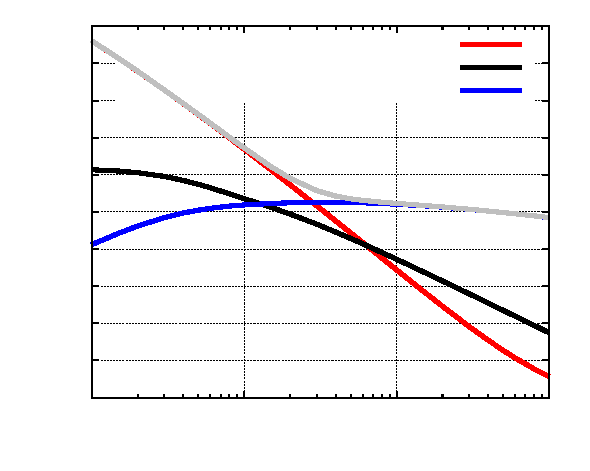
\includegraphics{AttenuationWater}}%
    \gplfronttext
  \end{picture}%
\endgroup

		\caption{The different contributions to the attenuation of water at room temperature and the total attenuation.}
		\label{fig:AttenuationWater}
\end{figure}

In fact, the attenuation cross-section $\sigma$ is dependent upon the several different mechanisms in which a X-ray photon interacts with the atomic electrons. The 3 most relevant effects are the photoelectron absorption, the coherent scattering and the incoherent scattering, which sum up to the total attenuation coefficient:

\begin{equation}
        \mu = \rho_e (\tau_{\text{abs}}+\sigma_{\text{scat, coh}}+\sigma_{\text{scat, incoh}})
\end{equation}

When the X-ray photon is completely absorbed by the atom, the event is called photoelectron absorption because a photoelectron with the excess energy is expelled from an inner atomic shell, leaving the atom ionized. The created core-hole is consequently filled by an electron from an outer shell either by a radiative process, i.e. \emph{fluorescence}, or by a non-radiative mechanism emitting a secondary electron, i.e. Auger effect. The photoelectric effect is the predominant contribution to the attenuation principally at low X-ray energies and the ultraviolet regime, as shown in figure \ref{fig:AttenuationWater}. 

The other relevant contributions at the X-ray range are related to scattering processes. In an inelastic scattering event, the energy of the incident photon is partially transfered to a loosely bond electron resulting in a scattered photon with a lower frequency, according to the Compton relation $\Delta\lambda = \sfrac{h}{m_e c}\left( 1 - \cos{\Theta} \right) $, where $\Theta$ is the scattering angle. The Compton scattering is incoherent and contributes generally less than the elastic scattering at energies below 10 keV, as observed in figure \ref{fig:AttenuationWater}. Besides, the coherent scattering signal is the summation of the constructive interferences of the electromagnetic wave, which produces a higher scattered intensity than the inelastic scattering. In fact, the elastic scattering of X-rays is the main proccess used in material investigations and the pyhsical principle behind SAXS.

\subsection{Elastic scattering}
\label{sec:ElasticScattering}

When the wavelength of the scattered wave is the same than that of the incident one, the proccess is named elastic scattering or coherent scattering and the resulting intensity is the absolute square of the sum of the scattering amplitudes. In the following sections, the elastic scattering theory will be presented for the classical case and for an ensemble of electrons.

\subsubsection{Thomson scattering}

Classically, the elastic scattering of a photon by a free electron is described by the conservation of the photon energy, i.e. the wavenumber of the scattered wave is the same than the incident one ($\abs{\vec{k_{\text{s}}}}=\abs{\vec{k}}$). Consequently for unpolarized incident radiation, the intensity of the scattered wave at a distance $r$ and with a scattering angle $2\Theta$ is defined by \citep{warren_x-ray_1969}:

\begin{equation}
        I_{\text{scat}}\left( r,\Theta \right)= I_0 \left( \frac{r_e}{r} \right) ^2 \left( \frac{1+\cos^2{2\Theta}}{2} \right)
\end{equation}

where $r_e= \sfrac{e^2}{4\pi\epsilon_0 m c^2}=2.82\cdot10^{-15}$ m is the Thomson or classical electron radius. A relevant quantity in scattering processes is the differential scattering cross-section $\sfrac{d\sigma}{d\Omega}$, which is defined as the the number of scattered photons per time and per solid angle over the incident intensity per time and per area:

\begin{equation}
        \label{eq:thomson_cross_section}
        \frac{d\sigma}{d\Omega}= \frac{I_{\text{scat}} \cdot \left(r^2 \Delta \Omega \right)}{I_0\Delta \Omega}=r_e^2\left( \frac{1+\cos^2{2\Theta}}{2} \right)
\end{equation}

where $r^2 \Delta \Omega$ is the detector surface in the plane of the impact parameter. The total Thomson scattering cross-section is $\sigma = \sfrac{8\pi r_0^2}{3} = 0.665\cdot10^{-24}$ cm$^2$ and similarly to $\sfrac{d\sigma}{d\Omega}$ is both proportional to $r_e^2$ and independent on the photon energy at the X-ray regime away of a resonant excitation.

\subsubsection{Scattering by an ensemble of electrons}

\begin{figure}%[htbp]
	\centering
	        \def\svgwidth{0.75\linewidth}
		\input{Figures/BeerLambertScheme.pdf_tex}
		\caption{Scheme of an scattering event at a position $\vec{r}$}
		\label{fig:FraunhoferScheme}
\end{figure}

The scattering of a photon by an ensemble of weak bounded electrons can be studied by considering the interaction of particles with a three-dimensional weak potential field $\phi(\vec{r})$. The resulting wave can be expressed as a linear combination of the incidient plane wave (see equation \ref{eq:IncidentWave}) and the scattered spherical wave at the position $\vec{r}$:

\begin{equation}
       \Psi\left( \vec{r} \right)= \Psi_0\left( \vec{r} \right) +  \Psi_{\text{scat}}\left( \vec{r} \right)
\end{equation}

Introducing this expression at the time-independent Schrödinger equation and considering the scattering wave as a perturbation produced by the scattering density function $\phi(\vec{r})$ \citep{cowley_diffraction_1995}, it can derived that

\begin{equation}
       \Psi_{\text{scat}}\left( \vec{r} \right)=C \int \frac{e^{ i \vec{k}\abs{\vec{r}-\vec{r}'} } } {\abs{\vec{r}-\vec{r}'}} \phi(\vec{r}')   \Psi\left( \vec{r}' \right) d\vec{r}'^3
\end{equation}

where $C$ is the so-called \emph{scattering length}. If the detection position $\vec{r}$ is at distance much larger than the scattering object size, as outlined in figure \ref{fig:FraunhoferScheme}, the Fraunhoffer approximation applies and $\abs{\vec{r}-\vec{r'}}=r$ \citep{feigin_structure_1987}, resulting in

\begin{equation}
       \Psi_{\text{scat}}\left( \vec{r} \right)=C \frac{e^{i k r}}{r} \int e^{ -i \vec{k}\vec{r}' }  \phi(\vec{r}')   \Psi\left( \vec{r}' \right) d\vec{r}'^3
\end{equation}

Assuming that there are no multiple scattering events due to the low concentration of scatterers and that the potential field is weak, the first Born approximation can be employed ($ \Psi\left( \vec{r} \right) \simeq \Psi_0\left( \vec{r} \right)$) \citep{cowley_diffraction_1995}, leading to

\begin{equation}
       \Psi_{\text{scat}}\left( \vec{r} \right)=C A_0 \frac{e^{i k r}}{r} \int e^{ i \vec{q}\vec{r}' }  \phi(\vec{r}')  d\vec{r}'^3
\end{equation}

where $\vec{q}=\vec{k_s} - \vec{k}$ is the momentum transfer vector and $\vec{k_s}$ the scattered wavevector. Analogously to equation \ref{eq:thomson_cross_section}, the differential scattering cross-section is:

\begin{equation}
        \label{eq:rayleigh_cross_section}
        \frac{d\sigma}{d\Omega}= \frac{\abs{\Psi_{\text{scat}}}^2 \cdot \left(r^2 \Delta \Omega \right)}{\abs{\Psi_{0}}^2\Delta \Omega}=r_e^2 \abs{f(\vec{q})}^2
\end{equation}
where $f(\vec{q})=\int e^{ i \vec{q}\vec{r}' }  \phi(\vec{r}')  d\vec{r}'^3$ is the scattering amplitude and the scattering length is the classical electron radius $r_e$. The scattering amplitude is simply the Fourier transform of the scattering potential field $\phi(\vec{r})$. 

This type of scattering mechanism is called Rayleigh-Gans-Debye when the refractive index of the object ($n_{\text{obj}}$) is close to unity and the condition $\sfrac{2\pi}{\lambda} \cdot a \cdot n_{\text{med}} \cdot \abs{1-\sfrac{n_{\text{obj}}}{n_{\text{med}}}}\ll1$ is fulfilled, being $a$ the size of the object. For X-ray photons with wavelenghts $\lambda$ in the Angstrom range and colloidal objects in the nanoscale, this approximation can be employed and it can be assumed that the same electromagnetic wave impinges each part of the object \citep{hulst_light_1957, barber_rayleigh-gans-debye_1978}. In the case of optical radiation on colloids, the Mie scattering framework is used, while the Rayleigh scattering corresponts to light wavelengths much larger than the scattering object.

\subsubsection{Anomalous scattering}

In X-ray scattering experiments, the scattering centers are the electrons of the atom and the scattering field is the electron charge density about the nucleous, so $\phi(\vec{r})=\rho_e(\vec{r})$. The electron density is related to the atomic properties as introduced in equation \ref{eq:AttenuationMultiComponent} and therefore the scattering amplitude increases with the atomic number $Z$ by calculating equation \ref{eq:rayleigh_cross_section} at the limit $\vec{q} \rightarrow 0$

\begin{equation}
        f(\vec{q} \rightarrow 0) = \int \rho_e(\vec{r}')  d\vec{r}'^3 = Z
\end{equation}

This is valid when the incident radiation energy is much greater than the energy corresponding to a resonant excitation. When the X-ray energy is close to an absorption edge, anomalous dispersions becomes relevant and the scattering amplitude depends on the energy of the X-ray by adding the anomalous corrections \citep{als-nielsen_elements_2011}:

\begin{equation}
        f(E) = f_0 + f'(E) + i f'' (E)
\end{equation}

where the imaginary part $f''$ is related with the attenuation coefficient $\mu$ by\citep{feigin_structure_1987}

\begin{equation}
        f'' (E) = \frac{A\rho}{2N_A r_0 h c} E \mu(E)
\end{equation}

where $A$ is the atomic mass of the resonant atom and $\rho$ its physical density. The term $f'$ is related to the imaginary part by the Kramers-Kronig relationship \citep{de_l._kronig_theory_1926,kramers_diffusion_1927}:

\begin{equation}
        f'(E) = \frac{2}{\pi} \int_0^{\infty} \frac{E'f''(E')dE'}{E^2 - E'^2}
\end{equation}

The values of the anomalous scattering amplitude $f(E)$ are usually calculated using the experimentally measured attenuation coefficient $\mu(E)$.

\section{Small-angle X-ray scattering}

Small-angle X-ray scattering is a powerful technique that can elucidate the structural features of particles with sizes ranging from about 2 nm up to 400 nm. By investigating the photons elastically scattered by the electron density distribution of the particle, the resulting patterns can be analysed according to equation \ref{eq:rayleigh_cross_section} to obtain information about the particle size, shape and composition. The fundamental quantities in a SAXS experiment are the scattering intensity $I(\vec{q}) = \abs{f(\vec{q})}^2$ and the scattering amplitude or \emph{form factor} $f(\vec{q})$, that for objects with spherical symmetry ($\rho_e(\vec{r})=\rho_e(r)$) is expressed by

\begin{equation}
        \label{eq:FormFactorSpherical}
        f(q)=4\pi \int_0^{\infty} r'^2 \rho_e(r')  \frac{\sin(qr')}{qr'}  dr'
\end{equation}

where the modulus of the momentum transfer vector is defined by $q=\abs{\vec{q}}=\abs{\vec{k_s} - \vec{k}}$. Considering that SAXS is an elastic scattering proccess ($\abs{\vec{k_s}}=\abs{\vec{k}}=\sfrac{2\pi}{\lambda}$), the momentum transfer is expressed as

\begin{equation}
q=\frac{2\pi }{\lambda}\sin\theta=\frac{4\pi E}{h c}\sin\theta ,
\end{equation}

where \(\theta\) is half of the scattering angle as depicted in figure \ref{fig:FraunhoferScheme}, \(h\) is the Planck constant and \(c\) is the speed of light.

The systems studied by SAXS in this work consist of particles suspended in a uniform medium, e.g. water or buffer, with a different electron density $\rho_{\text{medium}}$ than the studied particle. In fact, the measured scattering amplitude is the addition of the medium and the particle contributions. Therefore, the scattering of the studied object is expressed in terms of the \emph{contrast}, $\Delta \rho (\vec{r}) = \rho_e(\vec{r}) - \rho_{\text{medium}}$, the electron density difference between the particle and the embedded matrix or surrounding medium. This leads to a slight modification of equation \ref{eq:FormFactorSpherical}, where $\rho_e(r)$ can be substituted by the contrast $\Delta\rho(r)$ to distinguish the contribution from the investigated particle from the medium.

\subsection{Scattering by an ensemble of particles}

For diluted systems with low particle concentration, the wave scattered by a particle does not interfere coherently with the neighboring particles and the scattering intensity can be expressed as a sum of the individual scattering, i.e. the structure factor contribution can be neglected because $S(q)=1$\citep{feigin_structure_1987}. Therefore, the scattering intensity of an ensemble of randomly oriented nanoparticles in a diluted suspension can be expressed as

\begin{equation}
\label{eq:intensity}
I(q)=N\int_{0}^{\infty} g(R)\left|f(q,R) \right|^2 dR,
\end{equation}

where \(N\) is the number of scatterers i.e particles, \(g(R)\) is their size distribution function and \(f(q,R)\) is the particle form factor, which depends on the radial structure of the particle as determined in equation \ref{eq:FormFactorSpherical}. Generally, the particles in suspension are not monodisperse show a certain size distribution which is directly related with their chemical preparation. For systems of relatively low size polydispersity, a gaussian size distribution is typically a good choice, which is expressed by:

\begin{equation}
       g_{\text{Gauss}}(R)=\frac{1}{\sigma \sqrt{2\pi}} e^{ - \frac{\left( R - \mu \right)^2}{2\sigma^2} }
\end{equation}

where $\mu$ is the mean size of the particles and $\sigma$ is the standard deviation of the size distribution. For smaller particles or higher polydispersity degrees, a log-normal distribution is preferred, defined as

\begin{equation}
       g_{\text{LN}}(R)=\frac{1}{\sigma \sqrt{2\pi}} e^{ - \frac{\left( \ln(R) - \ln(\mu) \right)^2}{2\sigma^2} }
\end{equation}

whose mean size is given by $\mu e^{\frac{\sigma^2}{2}}$ and the variance is $\mu^2 e^{\sigma^2} (e^{\sigma^2} - 1)$. Other approaches to the size distribution of particles in solution are based in numerical techniques, like the Monte-Carlo approach to form-free particle size distributions \citep{pauw_improvements_2013}.

\subsection{What is measured in a scattering experiment?: The scattering curve}

The differential scattering cross-section $\sfrac{d\sigma}{d\Omega}$ is the fundamental measurand in a SAXS experiment, as described in section \ref{sec:ElasticScattering}. Nevertheless, some comparability challenges arise from this quantity as it depends on the sample volume used in the experiment. Therefore, the differential scattering cross-section per volume is introduced, historically given in cm$^{-1}$. The expression of this quantity is derived from equations \ref{eq:rayleigh_cross_section} and \ref{eq:intensity} and leads to:

\begin{equation}
        \frac{d\Sigma}{d\Omega} (q) = \frac{\sfrac{d\sigma}{d\Omega}}{V} (q) = r_e^2 \cdot \frac{N}{V} \cdot \int_0^{\infty} g(R) \abs{ f(q,R) }^2 dR
\end{equation}

where $\sfrac{N}{V} = C$ is the concentration of scatterers, i.e. particles

The scattering curve is the typical form to present the experimental data, which displays the differential scattering cross-section per volume versus the momentum transfer $q$ in a log–log graph. Three different regions can be distinguished in a scattering curve \citep{schnablegger_practical_2006}: 

\begin{itemize}
        \item The \textbf{Guinier region} comprises the low-$q$ region where $qD<1.3$\citep{feigin_structure_1987}, being $d$ the characteristic length of the investigated object. This region provides principally information about the size of the particle
        \item The high-$q$ region is called the \textbf{Porod region}, where information about the surface-to-volume ratio of the particles can be derived. For a smooth particle surface, the scattering intensity decays as $q^{-4}$, while for rough or fractal surfaces the slope is a function of $q^{-b}$ with $2<b<4$ \citep{walenta_small_1985-1}.
        \item For sufficiently monodisperse particle suspensions, the \textbf{Fourier region} or middle-$q$ region of the scattering curve shows pronounced minima that characterize the particle structure and shape.

\end{itemize}

\subsection{Modelling of the scattering intensity: Form factors}

Besides the information from the size distribution of the particle ensemble, the modelling of the scattering intensity $I(q)$ provides very precise information about the shape and composition of the particles by modelling the form factor or scattering amplitude. In the simple case of a solid sphere with uniform density $\rho_0$, the radial electron density profile is described by $\rho_e(r>R)=0$ and $\rho_e(r<R)=\rho_0$, whilst the integral of expression \ref{eq:FormFactorSpherical} is limited to the radius of the particle $R$. The form factor of a homogenous solid sphere is 

\begin{equation}
       f_{\text{sph}}(q,R)=\frac{4}{3}\pi R^3 \left( \rho_0 - \rho_{\text{medium}} \right) \left( 3\frac{\sin(qR)-qR\cos(qR)}{\left( qR \right)^3} \right) = \Delta \rho_0 \cdot F_{\text{sph}}(q,R)
\end{equation}

where $\Delta \rho_0$ is the excess electron density or contrast and $ F_{\text{sph}}(q,R)$ is defined for convenience. 

Generally, nanoparticles show an internal heterogeneity and an inner electron density distribution. If the components are radially distinguishable, the form factor of a typical morphology with sharp interfaces between the radial symmetric components of the particle with radius \(R_i\) is

\begin{equation}
\label{eq:multicore-shell}
f\left(q,R \right)= \Delta \eta F_{\text{sph}}(q,R)+\sum_{i=1}^{n-1} \Delta\rho_i \left( F_{\text{sph}}(q,R_{i+1})-F_{\text{sph}}(q,R_{i}) \right) ,
\end{equation}

where \(R\) is the external radius of the particle and \( n \) is the number of concentric shells. The excess of electron density of each component is $\Delta\rho_i = \rho_i - \rho_{\text{core}}$ and the contrast is defined in this case as $\Delta \eta = \rho_{\text{core}} - \rho_{\text{medium}}$ in order to isolate the solvent electron density in one term.

The simplest case of expression \ref{eq:multicore-shell} arises for core-shell particles. This model represents a radially symmetric particle with a sharp interface between the outer shell and the inner core. The form factor is described by

\begin{equation}
        \label{eq:ff_cs}
	f_{\text{CS}}(q,R)=  \Delta\eta F_{\text{sph}}(q,R) +  \Delta\rho\left[ F_{\text{sph}}(q,R)-F_{\text{sph}}(q,R_{\text{core}}) \right] ,
\end{equation}

where \(R \) and \(R_{\text{core}} \)  are the outer shell and inner core radii respectively, the excess of electron density is \(\Delta\rho=\rho_{\text{shell}}-\rho_{\text{core}}\) and the contrast is expressed as \(\Delta\eta=\rho_{\text{core}}-\rho_{\text{solv}}\), where $\rho_{\text{solv}}$ is the electron density of the suspending medium.

Depending on the synthesis of the particles, the interface between the different phases might show a linear gradient of the electron densities of the components. Analogously to expression \ref{eq:multicore-shell}, the form factor of a multicomponent spherical particle with a linear gradient interface is

\begin{equation}
f\left(q,R \right) = \sum_{i=0}^{n-1}\left[m_i \left( F_{\text{lin}}(q,R_{i+1})-F_{\text{lin}}(q,R_{i}) \right) +b_i \left( F_{\text{sph}}(q,R_{i+1})-F_{\text{sph}}(q,R_{i}) \right) \right]
\end{equation}
where $m_i=\sfrac{\left( \rho_{i+1}-\rho_{i} \right)}{\left( R_{i+1}-R_{i} \right)}$ and $b_i=\left( \rho_i-\rho_{\text{solv}} \right)-R_im_i$ and the linear form factor is defined by
\begin{equation}
F_{\text{lin}}(q,R) = 4\pi\frac{ \left( 2qR\sin(qR)+2\cos(qR)-(qR)^2\cos(qR) \right)}{q^4}
\end{equation}

The presented form factors result from the models used in this work to analyze the experimental SAXS data of polymeric colloids in suspension presented in chapters \ref{chap:density_gradient_SAXS} and \ref{chap:simultaneous_size_density}.

\section{Contrast variation}

In the contrast variation method, the electron density of the particle or the surrounding medium is systematically altered in order to obtain independent scattering curves with different contrasts $\Delta \rho (r)$. This technique is useful to characterize the different components of a heterogenous particle, due to the complementary data that can be collected with this approach. In the work presented in this thesis, only the electron density of the suspendin medium is varied, using the so-called \emph{solvent contrast variation} method.

\begin{figure}%[htbp]
	\centering
	        \def\svgwidth{0.75\linewidth}
		\input{Figures/BeerLambertScheme.pdf_tex}
		\caption{Schematic representation of the variation of the solvent electron denstiy until matching the electron density of one of the particle's components}
		\label{fig:ContrastScheme}
\end{figure}

By means of the solvent contrast variation approach, the electron density of a single phase of the investigated particle can be matched, resulting in a increased scattering amplitude of the other components of the object, as depicted in figure \ref{fig:ContrastScheme}. This effect is called the \emph{match point} and enables a much more detailed study of the different contributions of the particle's components to the scattering intensity. In the following paragraphs, the theoretical framework needed to interpret a SAXS contrast variation experiment will be presented, focusing mainly on the variation of the solvent electron density $\rho_{\text{solv}}$.

 
\subsection{Isoscattering point}
One of the best known features appearing in a contrast variation experiment is the existence of \emph{isoscattering points}. At these specific \( q\)-values, the scattering intensity is independent of the adjusted solvent contrast, i.e. all scattering curves intersect in the isoscattering points regardless of the contrast. The isoscattering points \(q^{\star}\) are particularly interesting because they emerge for any spherical particle with an inner structure and a sufficiently narrow size distribution. From the contrast-depending part of equation \eqref{eq:multicore-shell}, a model-free expression can be derived which relates the position of the isoscattering points \(q^{\star}_i\) with the external radius of the particle \( R \), independent of its radial structure \cite{kawaguchi_isoscattering_1992}:

\begin{equation}
        \label{eq:isoscattering}
        \tan(q^{\star}_iR)=q^{\star}_iR
\end{equation}

The solutions for this equation fullfill $q^{\star} R =4.493, 7.725, 10.904, ...$, where the positions of the isoscattering points correspond to the minima positions of the scattering intensity of a compact spherical particle with radius \( R \). 

Although this expression is derived for the monodisperse case, it can still be applied up to a moderate degree of polydispersity, if care is taken regarding the shift of the minima position due to polydispersity \cite{beurten_polydispersity_1981}. If defining the polydispersity degree \( p_d\) as the full width half maximum of the particle size distribution divided by its average value, for size distributions with \( p_d\) larger than \( \approx 30\,\% \), the isoscattering point is not well defined and the intersection point of the curves is smeared out, showing a diffuseness in the isoscattering point position \cite{kawaguchi_isoscattering_1992}.

Similarly, any deviation from the spherical shape produces a diffuseness in the $q^{\star}$ position. Unfortunately, this effect cannot be distinguished from the smearing produced by the size polydispersity and the investigation of the particle shape needs to be perfomed by other means.


\subsection{Basic functions approach}
When analyzing contrast variation data, a widespread theoretical approach is based in the non-interacting model proposed by Stuhrmann $\&$ Kirste (\citeyear{stuhrmann_elimination_1965,stuhrmann_elimination_1967}) for monodisperse particles. The so-called \emph{basic functions} formulation differentiates, independently of the particle inner structure, the contributions which depend on the varying solvent density or contrast (\(\Delta\eta\)) and on the excess of electron density of each component of the particle. 

Deriving from this approach, the scattering intensity can be expressed as the combination of contributions corresponding to different features of the particles:
\begin{equation}
\label{eq:intensity_contrast}
I(q)=I_c(q)+\Delta\eta I_{sc}(q)+(\Delta\eta)^2 I_{s}(q)
\end{equation}
The $I_c$ function contains the contributions from the density fluctuations inside the particle, the contribution $I_s$ is the so-called \emph{resonant term} and $I_{sc}$ is the cross-term function.


\subsubsection{Shape factor}
The $I_s(q)$ function, also known as \emph{shape factor}, corresponds to the scattering contributions from particles with homogenous density and a size equivalent to the volume inaccessible to the solvent. By modelling the shape factor function, the shape and size distribution of the particles can be determined independently of their inner structure.

For different solvent densities

\begin{equation}
        A_{m,n} = 
 \begin{pmatrix}
  1 & \Delta \eta_1 &  \left( \Delta \eta_1 \right)^2 \\
  \vdots  & \vdots  & \vdots  \\
  1 & \Delta \eta_N &  \left( \Delta \eta_N \right)^2 
 \end{pmatrix}
        \cdot A      
 
\end{equation}

\subsubsection{Guinier approximation}
\label{sec:TheoryGuinier}

The radius of gyration of a particle about its center of mass $R_g$ is defined as the second moment of the electron density distribution and can be calculated by 

\begin{equation}
        R_g^2 = \frac{\int \rho (r) r^2 dr}{\int \rho (r)  dr}
\end{equation}

The radius of gyration is systematically employed in small-angle scattering as an evaluation tool, due to its applicability to a large diversity of sample, e.g. proteins, colloids, suprastructures \cite{mertens_structural_2010,sim_salt_2012}. If the object is spherical, the gyration radius is directly related with its external radius by $R_g^2 = \sfrac{3}{5}R^2$.

In SAXS, $R_g$ can be calculated using the Guinier approximation \cite{guinier_diffraction_1939,guinier_small-angle_1955}, which assumes that the scattering intensity behaves in the limit of small \(q\) as

\begin{equation}
\label{eq:guinier}
I(q) \simeq I(0)\,\mbox{exp}\left(-\frac{R_g^2}{3}q^2\right),
\end{equation}

where \( I(0)\) is known as forward scattering or intensity at zero angle. Using the basic functions approach, the radius of gyration of a monodisperse, heterogeneous particle can be expressed as a function of the solvent electron density \( \rho_{\text{solv}} \) and the average electron density of the particle \( \rho_0 \) \cite{feigin_structure_1987}
\begin{equation}
R_g^2=R_{g,c}^{\,2}+\frac{\alpha}{\rho_0-\rho_{\text{solv}}}-\frac{\beta}{(\rho_0-\rho_{\text{solv}})^2},
\label{eq:gyration}
\end{equation}
where \(R_{g,c}\) is the radius of gyration of the particle shape corresponding to the volume inaccessible for the solvent \( V_c \), \( \alpha \) characterizes the distribution of different phases inside the particle and \( \beta>0 \) considers the eccentricity of the different scattering contributions \cite{stuhrmann_small-angle_2008}. Nevertheless, particle aggregation influences the scattering curves especially in the Guinier region and must be explicitly avoided.

\cite{avdeev_contrast_2007} proposed an extended version to equation \eqref{eq:gyration} for the case of a polydisperse particle ensemble by introducing the \emph{effective} values \( \tilde R^2_{g,c} \), \( \tilde \alpha \) and \( \tilde \beta \), which are the intensity-weighted averages of the corresponding parameters over the polydispersity. The observed average electron density is not affected by the polydispersity (\( \tilde\rho_0=\rho_0 \)) if the volume ratio between the different particle components is constant for all particles in the ensemble.

Assuming the same premise, the intensity at zero angle is given by
\begin{equation}
\label{eq:I0}
I(0)\propto N \left( \rho_0-\rho_{\text{solv}} \right)^2 ,
\end{equation}
with a minimum at \( \rho_{\text{solv}}=\rho_0 \). Therefore, by analyzing the Guinier region of the scattering curves, the average electron density of the particle can be obtained without assuming an \emph{a priori} inner structure.

Using the models presented above, it is possible to obtain by independent means the external radius and the average electron density of the particle in suspension.
\subsubsection{$I(0)$}
what happens in polydisperse systems?

